%!TEX root = ../template.tex
%%%%%%%%%%%%%%%%%%%%%%%%%%%%%%%%%%%%%%%%%%%%%%%%%%%%%%%%%%%%%%%%%%%
%% chapter1.tex
%% NOVA thesis document file
%%
%% Chapter with literature review
%%%%%%%%%%%%%%%%%%%%%%%%%%%%%%%%%%%%%%%%%%%%%%%%%%%%%%%%%%%%%%%%%%%

\typeout{NT FILE literature_review.tex}%

\chapter{Literature Review}
\label{cha:literature review}


% epigraph configuration
\epigraphfontsize{\small\itshape}
\setlength\epigraphwidth{12.5cm}
\setlength\epigraphrule{0pt}

\epigraph{
  Lucky is he who has been able to understand the causes of things. (Virgil 29 BC)
}

\section{Review on foundational causal inference concepts}
\label{sec:mkt_campaings_vouchers} 
Humanity has long been fascinated by the quest to understand the causes of events. From making offerings to the gods in hopes of altering the
weather to deciphering whether a newly developed vaccine can prevent a disease and save humanity from a pandemic, the desire to uncover the
underlying causes of phenomena stretches back to antiquity.

For centuries, these causal questions lacked a formal framework for addressing causal questions. The traditional statistics fell short by failing to offer a proper
language to articulate or address these inquiries. However, the scientific landscape has undergone a transformation in recent decades with
the development of a new mathematical language and tools designed to express and answer these questions using data \parencite{pearl_causal_2016}.

\textcite{pearl_causal_2016} and \textcite{pearl_book_2020} highlight that the scientific community has recently experienced a "causal revolution",
the effects of which have permeated various fields, particularly the social and biomedical sciences. This is evidenced by the significant
increase in papers featuring the terms "causal" or "cause" in their titles, from 13 to over 100, at the 2003 Joint Statistical Meeting in
San Francisco, between 2003 and 2014.

Over the past four decades, as \textcite{morgan_counterfactuals_2015} note, a counterfactual model of causality has emerged, offering a unified
approach to addressing causal questions. This model, centered around the potential outcomes framework, serves as a foundational piece for 
engaging with causality and is introduced at the outset of this chapter. Subsequent sections will delineate the main assumptions supporting
causal inference, examining the ramifications of their violations on final estimations. The chapter concludes by discussing the nuances of
long-term experiments, pivotal for addressing the research questions of this thesis.

\subsection{The potential outcomes framework}
\label{sub:potential_outcomes_framework}

Causality is a pivotal concept in philosophy, attracting extensive discourse among thinkers regarding its nature and expression. The notion 
that one event triggers another presents a multitude of perspectives, this may impose an aditional chalange in the development of a standardized 
language for framing and addressing causal inquiries. \textcite{hume_enquiry_1993}, for example, depicted causality as a chronological sequence of events, where a 
preceding event directly causes the subsequent one. Conversely, \textcite{mill_system_2020} introduced five methodologies for determining 
causality, special attention to the difference method, which interprets causality through the lens of counterfactual comparisons. This method notably 
relates the potential outcomes framework, which currently predominates in tackling causal questions.

When it comes to statistics, the first main jump into inferring causal effects from data came with the development of one extremely powerful tool,
the Ordinary Least Squares (\Gls{OLS}) estimator. This tool, which is widely used in econometrics, was first derived by Gauss in 1809, with his works
to develop a method to predict the location of celestial bodies \parencite{gauss_c_f_theoria_1809}. Many other scientistis have contributed to the development
of \gls{OLS} in the following years, such as Legendre, Laplace, and others. As very well pointed out by \textcite{cunningham_causal_2021}, a very interesting
case and one of the first one of an application of \gls{OLS} in social sciences was made by \textcite{yule_investigation_1899} when he tried to 
understand if public assistance increased the number of mendicants in England, as an attempt to understand the causes of poverty. Eventhough his work
consisted into an important step into causal inference, it was an example of a naive application of \gls{OLS} to infer causal effects, as he did not
consider the possibility of other factors (even unobservable ones) that could have influenced, at the same time, the number of mendicants and the public assistance.
Such type of factores are called counfounders, and they tend to impose a severe problem in inferring causal effects, whichs is better discussed in the following sections.

When examining statistics, the pioneering leap towards deducing causal effects from data was marked by the advent of the Ordinary Least Squares
(OLS) estimator. This instrument, extensively employed in econometrics, originated from Gauss's efforts in 1809 to devise a method for 
predicting the positions of celestial bodies \parencite{gauss_c_f_theoria_1809}. Subsequent enhancements to OLS were made by scientists like 
Legendre and Laplace, among others. As highlighted by \textcite{cunningham_causal_2021}, an intriguing early application of OLS in the social 
sciences was conducted by \textcite{yule_investigation_1899}, who investigated whether public assistance contributed to an increase in 
mendicancy in England, aiming to explore the roots of poverty. Although his study represented a significant stride in causal inference, it 
exemplified a simplistic use of OLS for causal deduction, failing to account for other variables, including unseen ones, that might concurrently
affect the number of mendicants and public assistance levels (the outcome and treatment, respectively). These variables, known as confounders, pose a critical challenge in causal effect
determination, a topic better explored int the subsequent sections.

A pivotal progression in causal inference was the introduction of physical randomization of treatment among units. Although Splawa-Neyman suggested 
this approach in 1923 \parencite{splawa-neyman_application_1990}, its was not consider strictly necessary. It wasn't until Fisher's work \parencite{fisher_statistical_1992} 
that randomization was deemed crucial for causal inference, and further solidified as the gold standard in \textcite{fisher_design_1935} for addressing causal 
questions. Subsequently, numerous large-scale experiments were conducted across various fields, including medicine, agriculture, and business. 
Notable examples include the Public Health Service's study in 1954 to evaluate the Salk vaccine's effectiveness against polio and the RAND Corporation's 
research in the 1970s investigating health insurance's impact on healthcare utilization. To this day, physical randomization remains the most 
reliable method for causal inference. The underlying reason, which is discussed in more detail in subsequent sections, relates to its ability 
to ensure that treatment and control groups are comparable in all respects except for the treatment itself, a critical prerequisite for deducing 
causal effects.

Despite these advancements, a significant obstacle remained: the absence of a mathematical language to articulate causal questions. This gap represented an
important barrier to the development of causal inference methods for more complex scenarios, such as the ones where randomization is not possible. The breakthrough came in the 1980s 
with the development of the potential outcomes framework. Initially introduced by Splawa-Neyman in 1923 \parencite{splawa-neyman_application_1990}, it was later solidified by \textcite{rubin_estimating_1974}, 
offering a mathematical foundation to express and address causal questions, thereby overcoming a major hurdle in the field.

The potential outcomes has a simple, yet powerfull, idea. It consists on expressing the impact on a given outcome of interest as a comparison between two different state of the world: one
where the unit of interest is treated according to a given treatment and another one where it is not. Those two antagonsitic states are also called contrafactuals, and it represents
the outcome of the same individual in the same point of time, which makes the comparison between those two states an immpossible task, since both conterfactuals can never be oberserved.
When an action is taken, one potential outcome can be observed yet the other one is lost, this represents what is called the fundamental problem of causal inference, and it is the main
reason why causal inference is such a hard task to perform.

The potential outcomes framework embodies a straightforward yet potent concept. It articulates the effect on a desired outcome by contrasting two distinct "state of world": one where the unit 
in question receives a specific treatment, and another where it does not. These contrasting states, also known as counterfactuals, represent the outcomes for the same individual at the same point 
in time, making direct comparison challenging because both counterfactuals cannot be observed simultaneously. Once an action is taken, it is possible to observe one potential outcome, but the other becomes
inaccessible. This dilemma is known as the fundamental problem of causal inference, and it is the mainreason why causal inference is such a hard task to perform.

To get more practical, the potential outcomes framework can be expressed as follows, according to a binary treatment (either treated or not treated): Let $Y_i^1$ be the potential
outcome of unit $i$ if it is treated, and $Y_i^0$ be the potential outcome of unit $i$ if it is not treated. The causal effect of the treatment on unit $i$
is then defined as :

\begin{equation}
\updelta_i = Y_i^1 - Y_i^0
\label{eq:causal_effect}
\end{equation}

Now, $Y_i$ represents the observed outcome of unit $i$, and it is defined as:
\begin{equation}
 Y_i = D_iY_i^1 + (1 - D_i)Y_i^0
\label{eq:switching_equation}
\end{equation}

Where $D_i$ is the treatment indicator, which is equal to 1 if the unit is treated and 0 otherwise. The equation \ref{eq:switching_equation} is called the switching equation, and it represents
the observed outcome as a combination of the potential outcomes. Equations \ref{eq:causal_effect} and \ref{eq:switching_equation} represents what is called 
the fundamental problem of causal inference ,\parencite{holland_statistics_1986}. From those two equations it is possible to see that $\sigma_i$ is impossible to obtain.  

As pointed out by \textcite{morgan_counterfactuals_2015} : "The fundamental problem of causal inference requires that we focus on non-individual
level causal effects, maintaining assumptions about treatment assignment and treatment stability that will allow us to give causal interpretation to
differences in average values of observed outcomes", it is a tradition in the potential outcomes framework to focus on different types of causal averages.

The first one and the most famous is the average treatment effect (\gls{ATE}). It is defined as the average difference between the potential outcomes of the treated and the untreated units, as shown above:

\begin{equation}
\begin{aligned}
E[\updelta] = E[Y_i^1 - Y_i^0] \\
= E[Y_i^1] - E[Y_i^0]
\label{eq:ATE}
\end{aligned}
\end{equation}

Notice that even in the equation \ref{eq:ATE}, the fundamental problem of causal inference persists, since both potential outcomes
are still required on unit level. 

The next one, following pretty much the same idea, is the average treatment effect on the treated (\gls{ATT}). It is defined as the average difference 
between the potential outcomes of each of the treated units. It is defined as:

\begin{equation}
\begin{aligned}
E[\updelta|D_i = 1] = E[Y_i^1 - Y_i^0|D_i = 1] \\
= E[Y_i^1|D_i = 1] - E[Y_i^0|D_i = 1] \\
\label{eq:ATT}
\end{aligned}
\end{equation}

The last one, and the less famous, is the average treatment effect on the untreated (\gls{ATU}). It is the counterpart of the \gls{ATT}, and it is defined as the average difference
between the potential outcomes of each of the untreated units. It is defined as:

\begin{equation}
\begin{aligned}
E[\updelta|D_i = 0] = E[Y_i^1 - Y_i^0|D_i = 0] \\
= E[Y_i^1|D_i = 0] - E[Y_i^0|D_i = 0]
\label{eq:ATU}
\end{aligned}
\end{equation}

With all these concepts stablished, it is easy to see that \gls{ATE} is the weighted sum of the \gls{ATT} and the \gls{ATU}, and it is defined as:

\begin{equation}
  ATE = \pi ATT + (1 - \pi)ATU
  \label{eq:ATE_ATT_ATU}
\end{equation}

Where $\pi$ is the proportion of treated units in the population. It is important to note that \gls{ATE} is not necessarily equal to \gls{ATT} or \gls{ATU} since the characteristics
of treated units can differ from those of the untreated ones, and their responses to the treatment can also vary. This is a common scenario, especially in observational studies where
the treatment is not randomly assigned, and the assignment to treatment is based on the observed characteristics of the units instead. This phenomenon is referred to as selection bias
, and it is more thoroughly discussed in the sections that follow.

Until now, the potential outcomes framework has been presented in a very simple way, but impossible to calculate in practice. A naive attempt to 
estimate the \gls{ATE} from data would be to calculate the difference between the average observed outcomes of the treated and the untreated units : 

\begin{equation}
\begin{aligned}
  SDO = \bar{Y}^1 - \bar{Y}^0 \\
  = E[Y_i^1 | D = 1] - E[Y_i^0 | D = 0] \\
  = \frac{1}{n_1}\sum_{i=1}^{n_1}(Y_i^1 | D_i = 1) - \frac{1}{n_0}\sum_{i=1}^{n_0}(Y_i^0 | D_i = 0)
  \label{eq:SDO}
\end{aligned}
\end{equation}

The simple difference of means, or simple difference of outcomes (\gls{SDO}), is an estimator that can be directly estimated from the data, since 
it does not require to know both potential outcomes for each individual unit. However, it is not a consistent estimator for the \gls{ATE},
in order to see why, the following equation decomposes the \gls{SDO} into relevant components : 

\begin{equation}
\begin{aligned}
  E[Y_i^1 | D = 1] - E[Y_i^0 | D = 0] = ATE +  \\
                                      + (E[Y_i^0 | D = 1] - E[Y_i^0 | D = 0]) \\ 
                                      + (1 - \pi)(ATT - ATU) \\ 
  \label{eq:SDO_decomposition}
\end{aligned}
\end{equation}

From the equation \ref{eq:SDO_decomposition}, it is possible to see that the \gls{SDO} is a biased estimator for the \gls{ATE}, since it is not only 
estimating the \gls{ATE}, but also two important factors : the selection bias and the treatment effect heterogeneity. 

The selection bias is the difference
between the treated group and the untreated group ($E[Y_i^0 | D = 1] - E[Y_i^0 | D = 0]$), had both of them not been treated. It sounds a bit complicated but,
basically, it is the inherent difference between both groups of units and it carries important information about the treatment assignment mechanism. The
other component, the treatment effect heterogeneity, represents how differently the both groups reacts to the treatment. Physical randomization would be a cleaver
attempt to solve those problems, by selecting units randomly to receive or not the treatment we garantee that there is no other factor that could influence the treatment
assignment, in other words, we garantee that the selection bias term from equation \ref{eq:SDO_decomposition} is zero, the same for the other bias term (treatment effect 
heterogeneity) since \gls{ATT} is the same as the \gls{ATU}.

One major insight derived from this naive estimation of \gls{ATE} is the fact that the treated and untreated groups can be inherently different due to factors that could, in the same time,
have  influenced the treatment administration and the outcome. Those factors are called counfounders, and taking them into consideration when estimating causal effects is a major challenge. 
The next sections will discuss the main assumptions that must be taken into consideration when analysing any causal question.

\subsection{Unconfoundedness}
\label{sub:uncounfoundedness}

As discussed earlier, the naive approach to estimating the \gls{ATE} from data can be biased due to the presence of confounders. As already pointed out, confounders are factors that are related to the treatment administration 
and the outcome simultaneously. In practice, most treatments, exposures, or actions intended to affect a given phenomenon are based on certain criteria. These criteria can be based on observable characteristics of 
individuals or even unobservable ones, given that human beings rarely act randomly. This poses the primary challenge when attempting to estimate causal effects from observational data: the treatment assignment 
process is not under the researcher's control, and understanding what motivates the treatment selection is the first step.

One of the main assumptions of causal inference has all to do with the presence of confounders, in fact its name , Unconfoundedness, is a direct reference to the required absense of confounders in the treatment estimation. This
assumptions states that the treatment must be independent of the potential outcomes :

\begin{equation}
  (Y_i^1, Y_i^0) \perp D_i
  \label{eq:uncounfoundness}
\end{equation}

In experimental settings, where treatment assignment is controlled (and typically randomized), the treatment is designed to be independent of the potential outcomes $Y_i^1$ and $Y_i^0$. When this condition is satisfied, the 
treatment assignment mechanism is often considered ignorable \parencite{morgan_counterfactuals_2015}.

It is crucial to note that equation \ref{eq:uncounfoundness} does not imply that the observed outcome $Y_i$ should be independent of the treatment; in reality, it is not. This relationship is evident in equation 
\ref{eq:switching_equation}, where the observed outcome is actually dependent on the treatment and the potential outcome corresponding to the realized treatment state.

The unconfoundedness assumption poses a significant challenge to observational studies because it is difficult to ensure that the treatment selection mechanism is fully accounted for. Thus, for social scientists and other researchers 
attempting to establish causal effects under these conditions, the initial step involves identifying a set of variables $W$ that may act as confounders. By achieving conditional independence between the treatment and potential outcomes, with all variables 
$W$ held constant (\textit{ceteris paribus}), the treatment effectively becomes randomly observed among the units, satisfying the unconfoundedness assumption:

\begin{equation}
  (Y_i^1, Y_i^0) \perp D_i | W_i
  \label{eq:uncounfoundness_conditional}
\end{equation}

To garantee the absence of any confounders is notably stringent and challenging to ensure in practical scenarios. Specifically, for this study, accounting for all factors influencing voucher distribution presents a considerable challenge. 
Moreover, even if the allocation mechanism were fully understood—a daunting task in a business context—it would likely follow a deterministic process. In such a process, units meeting specific criteria either receive vouchers or 
do not, leading to a significant problem: the lack of comparable individuals across differing treatment conditions. This relates to the next assumption : positivity.

\subsection{Positivity}
\label{sub:positivity}
In the preceding section, we discussed the conditional independence assumption, referred to as equation \ref{eq:uncounfoundness_conditional}. This assumption posits that within a certain covariate level 
$W$, the treatment assignment can be regarded as if it were random. Bearing this in mind, and following the guidance of \textcite{facure_causal_2023}, the conditional independence assumption (CIA) offers an alternative approach to estimating the Average Treatment Effect (\gls{ATE})
when these covariates are present:

\begin{equation}
ATE = \sum_{w} \left( E[Y|T=1, W=w] pr(W=w) - E[Y|T=0, W=w] pr(W=w) \right)
\label{eq:adjustment_formula}
\end{equation}

The adjustment formula, as indicated in Equation \ref{eq:adjustment_formula}, posits that the Average Treatment Effect (\gls{ATE}) can be calculated as the weighted average of the expected outcome differences between treated and untreated units, conditioned on a specific level of covariates 
$W$. The weights are determined by the prevalence of units within the population sharing the same covariate profile $W$.

Furthermore, the adjustment formula underscores the significance of the positivity assumption in causal inference. This assumption requires that every unit in the population, at each level of covariates  W, has a non-zero probability of receiving the treatment. Put simply, for all covariate 
$W$ within the population, the likelihood of treatment assignment must be positive and less than one:

\begin{equation}
  1 > Pr(D | W ) > 0
  \label{eq:positivity}
\end{equation}

Within the scope of this thesis, the positivity assumption is a significant concern, as business teams often follow a deterministic process to allocate vouchers among customers. Take, for example, the marketing teams at iFood who utilize the lifetime segmentation of a customers
to determine voucher distribution. Consequently, new users, labeled as 'prospects', are typically assigned one voucher strategy ($D_a$) while 'active' customers are allocated a different strategy ($D_b$). This procedure infringes upon the positivity assumption, as it renders it
impossible to observe the behavior of a new user who has not received the voucher, denoted as $P(D_b | W = prospect) = 0$, and the same applies to active users, for whom $P(D_a | W = active) = 0$

The positivity assumption, also referred to as the common-support or overlap assumption, intriguingly intersects with a well-acknowledged concept in statistics and machine learning: the curse of dimensionality. One might initially think that to control for unconfoundedness, simply
incorporating all conceivable covariates into the causal model would suffice, potentially covering all confounders. Nevertheless, as the model includes more variables, the likelihood of encountering a unit with a specific combination of covariates $W$ diminishes. This is because 
the number of potential covariate combinations grows exponentially with the addition of more variables, a phenomenon attributed to the curse of dimensionality. In such an extreme case, the positivity assumption would be compromised. This issue is crucial for the latest advances 
in causal inference, particularly in its integration with machine learning \parencite{damour_overlap_2021}. The relevance of this topic to the context of this thesis is further explored in Chapter 3.

At this juncture, it is evident that the two assumptions previously discussed (Unconfoundedness and positivity) impose severe conditions on the analysis of observational data. These assumptions explains why an experimental approach was selected to address the causal question in this thesis.
However, opting for an experimental design does not absolve one of further meticulous considerations. The following assumptions refers directly to the problem examined in this study and, as will be demonstrated, are applicable even in experimental settings.

\subsection{SUTVA and consistency}
\label{sub:sutva_and_consistency}

From equation \ref{eq:switching_equation}, it is evident that the observed outcome $Y_i$ coincides with the potential outcomes $Y_i^1$ or $Y_i^0$, contingent upon the treatment $D_i$. This establishes a direct link between the treatment and its potential outcomes. However, a complication 
arises when the potential outcome cannot be entirely accounted for by the received treatment, a scenario encapsulated by the \gls{SUTVA}. This concept is delved into in \textcite{rubin_randomization_1980} and \textcite{rubin_comment_1986}, wherein Rubin articulates \gls{SUTVA} as
theu stipulation that the potential outcome of any unit must be independent of:

\begin{itemize}
  \item The treatment assigned to any other unit, sometimes called externalities, spillover or network effects.
  \item The mechanism in which the treatment is administrated, called treatment diluition, consistency or "no-multiple-versions-of-treatment".
\end{itemize}

Generally, a definition of SUTVA that encompass both cases mentioned above is when the potential oucome (and, consequently, the causal effect) is a function of the treatment, \parencite{morgan_counterfactuals_2015}. 

\begin{equation}
  \updelta_i(d) = Y_i^1(d) - Y_i^0(d)
  \label{eq:sutva_violation}
\end{equation}

Notice that this equation reflects both interpretation presented of \gls{SUTVA}, since the function that connects the treatment and the potential outcome can be describe to incorporate the treatments assignment accross other 
individuals of the population or the mechanism of treatment assignment (lets call this for now on the version of the treatment). 

In instances where \gls{SUTVA} is violated due to network effects or externalities, the accuracy of causal effect estimation may be compromised, even 
when prerequisites such as unconfoundedness and positivity are satisfied. The underlying issue is the interdependence of units within each treatment group,
where outcomes of individual units are not isolated but influence and are influenced by the outcomes of others units. Consequently, the comparison of treated
and untreated groups fails to offer a reliable measure of causal impact, specifically because untreated groups may inadvertently experience the treatment
through their interactions with treated individuals. This leads to a potential underestimation of the causal effect as the untreated groups absorb
a portion of the treatment's causal influence, originally intended for the treated group.

When violations of \gls{SUTVA} cames from externalities the causal effect estimation becomes very challenging. The literature of vaccinations are the reference on this kind of situation, check \textcite{hudgens_toward_2008} for further deatails. 
One possible approach is to use models that can directly take the network into consideration, check \textcite{goldsmith-pinkham_social_2013}.

In the context of this study, the alternative interpretation of \gls{SUTVA}, specifically concerning the presence of multiple versions of a treatment or the principle of consistency, is particularly pertinent. This issue emerges when the mechanism for assigning treatment results in treated units being exposed to varying intensities or types of the treatment.
For instance, in the scenario being examined of vouchers incentives the treatment in question involves exposure to vouchers, with versions differing in aspects such as discount rates, frequency of voucher distribution, methods of communicating the vouchers to customers, among other factors. These nuances and their implications are more thoroughly examined in Chapter 3,
where the experimental data and the design of the experiment conducted for this dissertation are detailed.

The concept of consistency in causal inference is thoroughly examined within the realms of philosophy and causal inference literature, often in relation to the clarity of the causal question posed and the meticulous definition of the treatment \parencite{hernanCompoundTreatmentsTransportability2011}. This principle is predominantly linked with observational studies within 
the domain of causal inference, yet it remains a significant subject of discussion in randomized experiments as well. The importance of precision in formulating this causal question has been recently emphasized by experts across various fields, including statisticians, epidemiologists, and computer scientists \parencite{pearl_consistency_2010, hernan_does_2008, coleConsistencyStatementCausal2009}.
The consistency assumption is formally described as follows:

\begin{equation}
  Y_i = Y_i^a, \quad  \text{when }  A_i = a, \text{for all }  a \in A
  \label{eq:consistency}
\end{equation}

Where $A$ is the treatment and When there exist multiple versions of treatment, the equation \ref{eq:consistency} is not applicable, indicating a breach of the consistency assumption. In those kind of scenarios, where various versions are present within a specific level of treatment, \textcite{hernanCompoundTreatmentsTransportability2011} introduces the concept of a compound treatment. From what has already been declared 
of the treatment discussed in this thesis, it should be clear that it serves as an illustrative case of a compound treatment. Another example involves analyzing the impact of physical activity on coronary heart disease when defining physical activity as engaging in exercise for at least 30 minutes versus less than 30 minutes. In such cases, the diversity of versions associated with each level of
treatment becomes evident.

Defining versions of a treatment is not always straightforward. For instance, one might argue that taking a pill of a specific drug with the right hand instead of the left could constitute different versions of the treatment (taking the pill). Clearly, such distinctions should not influence the estimation of causal effects, but in other scenarios, the differences might not be so easily dismissed.
To address this complexity, the concept of treatment variation irrelevance is introduced. It states that the relationship between the many different possible versions of a treatment and the outcome is negligible. Therefore, one can estimate the causal effect on the treatment variable level without further concerns.

When such assumption cannot be assument, carefull considerations must be taken. One possible approach would be to consider each possible version as a treatment per se, but this alternative became inviable when (1) few sample is left for each versions (when the number of versions is large), (2) the versions are not well defined. \textcite{lanza_causal_2013} proposed an alternative to deal with such cases,
despite some information regarding the treatment versions are still needed. Another approach, suggested by \textcite{vanderweeleCausalInferenceMultiple2013} would be to redefine the consistency assumption by introducing additional notation to the treatment and version of treatment. In this approach, the autors suggest expressing the potential outcome for unit j as $Y_j(a, k^a)$, where $A$ is the
treatment set to $a$ and $K^a$ is the version of the treatment set to $k^a$. The consistency assumption under the treatment variation irrelevance is then defined as:

When it's not feasible to assume treatment-variation irrelevance, careful consideration is required. One approach might involve treating each version as a separate treatment entity, but this strategy becomes impractical when: (1) the sample size for each version diminishes due to a large number of versions, or (2) the versions are not clearly defined. \textcite{lanza_causal_2013} offered an alternative method to
manage such scenarios, although some information about the treatment versions remains necessary. Another strategy, put forward by \textcite{vanderweeleCausalInferenceMultiple2013}, involves redefining the consistency assumption by incorporating additional notation for the treatment and its versions. In this method, the authors propose representing the potential outcome for unit $j$ as $Y_j(a, k^a)$, where $A$ denotes
the treatment assigned to as $a$ and $K^a$ represents the version of the treatment assigned to as $k^a$. Under this framework, the consistency assumption, considering treatment variation irrelevance, is defined as:

\begin{equation}
  Y_{j}(a, k^{a}) = Y_{i}(a, k^{a}) = Y_{i}(a, \circ) = Y_j \quad \text{for all } j, a, \text{ and } k^{a}, k'^{a} \in K^{a}.
  \label{eq:treatment_variation_irrelevance}
\end{equation}

\textcite{vanderweeleCausalInferenceMultiple2013} proposes two types of compound effect designation with distinct particularities : (1) when treatment precedes the versions (treatment-then-version) and (2) when version preced the treatment, so the treatment is basically a coarsion of the many versions administrated.
It is possible to identify that the current context of this research falls within the treatment-then-version category, since the version (voucher value, voucher distribution frequency, etc..) is a direct consequence of the treatment allocation (has voucher).
With this concept in mind, only this first category of compound effect is explored in the following text. Another important consideration is that the multiple-versions of treatment scenario, under the treatment-then-version case, is firstly explored above under the optic of an observational study and derivations of to the 
randomized experiment context are latter explored. 

\textcite{vanderweeleCausalInferenceMultiple2013} delineates two distinct categories of compound treatment effects: (1) treatment-then-version, where the treatment is administered before the determination of its versions, and (2) version-precedes-treatment, wherein the treatment essentially aggregates various administered versions. 
Within the scope of this research, the treatment-then-version category is more applicable, as the versions (e.g., voucher value, voucher distribution frequency, and others) emerge as a direct result of the treatment allocation (i.e., receiving a voucher).

Given this framework, the discussion henceforth will focus solely on the first category of compound effect. It's crucial to note that the scenario of multiple treatment versions, in the context of treatment-then-version,
is initially approached from the perspective of an observational study, with subsequent extensions to randomized experimental settings being discussed later.

Three different cases of causal effect identifications, under these conditions, are presented : (1) the causal effect of comparing each version to another, (2) the effect of treatment on the treated and (3) the overall causal effect for a population. Before delving into each of this cases, some assumptions are made regarding the way the investigated
causal question of this reasearch is formulated. The first, as already pointed out, is that our treatment variable is declared as a compound treatment which the treatment preceded the possible versions. The second is that the versions of the treatment are not defined, this assumption is made upon the fact that many different conditions determined the treatment
and that each customer can move between different versions, within the same treatment level. This observations are better explained and discussed in chapter 3. 

For the illustration of those cases, the following causal diagram, also extracted from \textcite{vanderweeleCausalInferenceMultiple2013}, is presented: 

\begin{figure}[htbp]
  \centering
  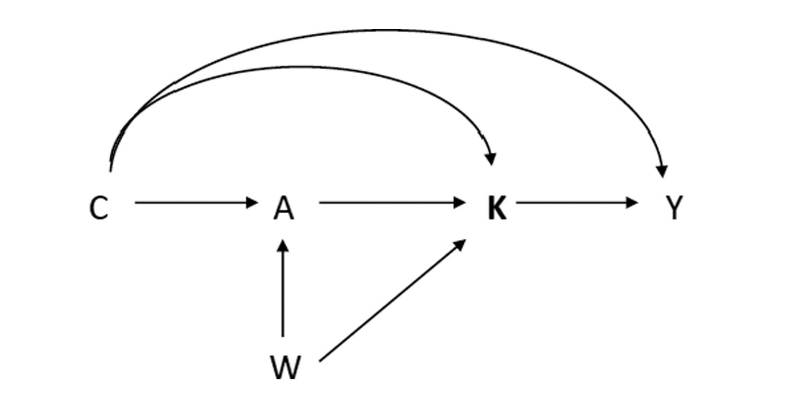
\includegraphics[height=2in]{multiple_versions_dag}
  \caption{Causal diagram illustrating the relationship between treatment $A$, version $K$ and different possible confounders $C$ and $W$, on outcome $Y$}
  \label{fig:causal_dag_multiple_versions}
\end{figure}

For the first case, the causal effect of comparing each version to another, only variable $C$ needs to be controlled in order to garantee the Unconfoundedness or exchangeability : 

\begin{equation}
  Y(a, k^{a}) \perp{{A,K} | C} \quad \text{for all } a \in A, k^{a} \in K^{a}
  \label{eq:condition_to_compare_versions}
\end{equation}

Equation \ref{eq:condition_to_compare_versions} represents the conditions in which states that it is not needed to control for the confounder between treatment and version (variable $W$), i.e for this particular case, it basically face the version and treatment combination as an unified treatment level.

To estimate the causal effect from data, of comparing treatment $a$ with $a*$ the following equation is used:

\begin{equation}
  \begin{aligned}
    E\{Y(a, k^{a})\} - E\{Y(a^{*}, k^{a^*})\} = \sum_{c} E\{Y|A = a, K^{a} = k^{a}, C = c\}pr(c) \\
     - \sum_{c} E\{Y|A = a^{*}, K^{a^*} = k^{a^*}, C = c\}pr(c).
  \end{aligned}
  \label{eq:causal_effect_compare_versions}
\end{equation}

Notice that equation \ref{eq:causal_effect_compare_versions} also relies upon the positivity, or common-support, assumption as it is needed a probability of bigger than zero and smaller
than one for each level of the confounder $C$.

The second case, the effect of treatment on the treated (\gls{ATT}) closely mirrors the first scenario regarding the variables that require control. The distinctive assumption here is the necessity of a singular,
possible version of the treatment under the control condition, denoted as $Y_i(0)$. The equation representing the \gls{ATT}, capturing the causal effect of the treatment on those treated, is articulated as follows:

\begin{equation}
  \begin{aligned}
    E\{Y(a, k^{a}) | A = a\} - E\{Y(0) | A = a\} = E(Y | A = a) \\
     - \sum_{c} E\{Y | A = 0, C = c\} \text{pr}(c | A = a).
  \end{aligned}
  \label{eq:causal_effect_treatment_treated}
\end{equation}

In this scenario, controlling for confounders between the treatment and its versions is not required. To apply equation \ref{eq:causal_effect_treatment_treated}, a less stringent
condition than \ref{eq:condition_to_compare_versions} suffices, specifically $Y(0) \perp {A,K^0} | C$. This indicates that under the control condition, 
the potential outcome $Y(0)$ is independent of both the treatment $A$ and the control version of the treatment $K^0$, given a set of covariates $C$.

For the last case, addressing the overall causal effect for the population, it's crucial to control for all confounders, represented as $W$ and $C$. 
\textcite{vanderweeleCausalInferenceMultiple2013} present evidence demonstrating that failing to control for a specific confounder $W$, which confounds 
the relationship between treatment and its version, can introduce bias into causal estimates.

In this context, the potential outcome under treatment $A=a$ is defined along with a function that specifies the version of the treatment: $Y(a) = Y(a, k^{a}(a))$.
To ensure Unconfoundedness and accurately estimate the causal effect, the conditional independence must be satisfied, which is articulated as follows:

\begin{equation}
  Y(a) \perp{{A}| {W,C}} \quad \text{for all } a \in A
  \label{eq:condition_to_overall_treatment_effect}
\end{equation}

A critical observation from equation \ref{eq:condition_to_overall_treatment_effect} is that, in scenarios where the treatment is randomized, as it is for
this study, the condition is inherently met. This is because randomization ensures the independence of the treatment from all other variables, effectively 
eliminating potential confounding factors. Under these circumstances, the causal effect between two distinct treatments can be accurately estimated using the following approach:

\begin{equation}
  \begin{aligned}
    E\{Y(a, k^{a}(a))\} - E\{Y(a^*, k^{a^*}(a^*))\} = \sum_{c,w} E(Y | A = a, C = c, W = w)\text{pr}(c, w) \\
     - \sum_{c,w} E(Y | A = a^*, C = c, W = w)\text{pr}(c, w).
  \end{aligned}
  \label{eq:causal_effect_overall_treatment}
\end{equation}

With all those three cases defined, the delineation of regimes and policies encapsulates key discussions on multiple versions of treatment within causal inference.
A regime represents a scenario where the combination of treatment and its versions formulates a new, distinct type of treatment. Here, both the treatment
and its versions are explicitly defined, serving together to frame a specific causal question. Conversely, a policy refers to instances where the versions 
of a treatment emerge from an undefined mechanism of treatment assignment, suggesting variability in how the treatment is applied across a population,\parencite{vanderweeleCausalInferenceMultiple2013}.

The concepts of regime and policy are particularly relevant to the context of this research, since the versions of the treament are not well defined. So the causal effect to be estimated
is related to the policy of voucher distribution on individuals purchase frequency. One important reflection that can be made regarding the relevance of estimating the causal effect of a policy 
instead of a regime, for this research theme, is that the regime can be faced as a deterministic process, where the versions of a given treatment follows a (hard to identify) combination of rules. Therefore,
those different possible forms of treatment administration are fixed and cannot be changed, whereas the treatment allocation (the voucher assignment) can be tailored and optimized.

The subsequent section delves into another vital aspect pertinent to this study: the challenges and unique characteristics of experimental designs extending over 
lengthy periods. Unlike their short-term counterparts, long-duration experiments introduce distinct considerations that must be addressed to ensure the validity and reliability of the causal estimates.

\section{Long term experiments}
\label{sec:long_term_experiments}

To estimate the long-term effects of voucher incentives on customer purchases, a six-month experiment will be utilized (with further details provided in the subsequent chapter).
Long-term experiments, unlike their short-term counterparts (one to two weeks), present unique challenges and characteristics. While short-term experiments are often adequate 
when the causal effect is stable and generalizes well over time, they may not accurately reflect long-term outcomes in cases where these conditions are not met.

This study addresses the gap between the long-term and short-term effects of voucher incentives. As mentioned in the introduction to the research question,
optimizing for short-term voucher investments may lead to a user dependency on voucher incentives, resulting in an unsustainable business model and marketing budget allocation.
Thus, conducting a long-term experiment to investigate these effects is essential.

The literature provides examples of the disparity between immediate and long-term effects. For example, a detrimental alteration to a search engine's algorithm
may initially lead to an increase in search queries due to users needing to search multiple times, but ultimately result in a long-term decline in query shares
\parencite{kohavi_trustworthy_2012}. Likewise, while increasing the number of advertisements on a website may boost click numbers in the short term, it could reduce
user engagement over the long-term  \parencite{hohnhold_focusing_2015}.

In \textcite{kohavi_trustworthy_2020} a comprehensive list of reasons of why long-term and short-term effect differs is presented, the ones that better connect with 
the research problem of this thesis are :

\begin{itemize}
  \item \textbf{User-learned effects} : Users can adapt to the treatment, making the effect of the treatment decrease over time. 
  For instance, in the case of vouchers incentives, users can learn that if they buy only when vouchers are given, the vouchers will keep
  appearing (as it can happen if the voucher's assingment method is only optimized to consider the immediate conversion as success),
  they can exploit this leading to a decrease of organic purchases in the long-term.
  \item \textbf{Seasonality}: The effect of the treatment can vary over time, for instance, in the case of vouchers incentives, 
  the effect of the vouchers can be different in the Christmas season or other comemorative dates.
\end{itemize}

An intuitive method for conducting and analyzing a long-term experiment involves measuring the treatment's effect in the initial week and again in the final 
week, then comparing the two. Although this approach may be feasible, it is crucial to consider several factors carefully. For this research problem, the primary 
concerns are survival bias and data leakage, which must be meticulously managed to ensure accurate and reliable results.

Survivalship bias is a form of selection bias that occurs when analyzing only the subjects that "survived" or made it to the end of a period, overlooking those that
did not. This can lead to skewed results and misleading conclusions. When analyzing long-term customer purchase frequency post-voucher incentive, if
we only consider customers who continue using iFood (the 'survivors'), we might overlook those who stopped using the service. This could falsely suggest 
that vouchers have a more positive or neutral long-term impact than they actually do.

To address survival bias, a recommended strategy, as outlined in \textcite{kohavi_trustworthy_2020}, involves conducting a cohort analysis. This approach entails
creating a stable cohort of users and examining both long-term and short-term effects exclusively within this group. The cohort should be established based on a stable
identifier, such as the user ID, and defined prior to the commencement of the experiment.

The leakage issue arises when user groups are inadvertently exposed to treatments or variants not intended for them, breaching the \gls{SUTVA} assumption
mentioned earlier. This violation can lead to underestimation of the actual treatment effect and dilute the treatment's exposure.

Addressing leakage is simpler compared to survival bias. Proper data analysis and cleaning can eliminate users who were inadvertently exposed to undesired experiment
variants.

The practical application of the strategies for handling both survival bias and leakage are further detailed in the following chapter, which discusses the data and its preprocessing steps.
As with any modeling approach, these preprocessing steps are crucial for ensuring result quality and are performed before modeling the conditional causal effect.

\section{Models for incentives allocation and Causal machine learning}
\label{sec:causal_inference_models_intro} 

Many causal inference techniques for observational and/or randomized data have been developed based on foundational concepts already introduced. The majority of these techniques focus 
on utilizing data in ways that make the treatment appear as if it were randomly generated, thereby addressing the issue of unconfoundedness. Key methods include:

\begin{itemize}
  \item \textbf{Ordinary Least Squares (OLS) Regression} : This method models the outcome using covariates and the treatment itself. It is one of the most traditional approaches and allows
   for estimating the impact of the treatment while accounting for the influence of multiple covariates.
  \item \textbf{Instrumental Variables (IV) and Two-Stage Least Squares (2SLS)} : This technique employs an instrumental variable that affects only the treatment, which may be biased due to 
  the presence of a confounder, and the outcome. It helps to isolate the causal effect of the treatment.
  \item \textbf{Difference-in-Differences (DiD)} : Utilizing panel data, this method compares the before-and-after outcomes of two populations with parallel trends, where only one receives the
   treatment. It effectively controls for time-invariant unobserved heterogeneity.
  \item \textbf{Regression Discontinuity Designs (RDD)} : This approach leverages the proximity to a cutoff point that motivates the treatment, comparing 
  individuals just above and below this threshold. It treats the treatment assignment as if it were randomly generated near the cutoff.
  \item \textbf{Matching} : This method compares individuals with similar covariates (i.e., those with the smallest distances between covariate vectors) who differ in treatment status. 
  It aims to create a balanced comparison group to estimate the treatment effect.
  \item \textbf{Propensity Score Matching (PSM)} : This technique models the probability of receiving the treatment and uses these probabilities (propensity scores) to match 
  treated and untreated individuals. It helps to ensure comparability between the two groups.
  \item \textbf{Doubly-Robust Estimation} : Combining propensity score estimates with outcome estimates (OLS) can suggest a doubly-robust method capable of handling situations where 
  either the propensity score model or the outcome model is misspecified. This approach enhances the robustness of causal effect estimation.
\end{itemize}

A review on those methods with practical applications can be found on \textcite{cunningham_causal_2021} and \textcite{morgan_counterfactuals_2015}. The last one, the Doubly-Robust Estimation is
a very curious one and is depicted carefully in \textcite{huber_causal_2023}.

These methods attempt to address confounder control in different ways to obtain unbiased causal effect estimates. However, a challenge arises when the number of variables to be considered is relatively 
large. In such cases, both inference (e.g., estimation of p-values) and the estimation of the causal effect (e.g., regression coefficients) are more susceptible to biases.

To address this problem, certain machine learning techniques are employed to handle high-dimensional spaces, allowing many variables to be included in the modeling process to control for potential confounders, 
provided there are no unmeasured confounders. One such technique is called doubly robust machine learning. As the name suggests, this method is robust to errors in both the estimation of the propensity score and 
the estimation of the conditional mean outcomes ($\mu(0)$, $\mu(1)$). This robustness arises from the fact that both are incorporated into the causal effect estimation multiplicatively. Consequently, errors in the 
estimation of one component are significantly offset by small errors in the other component. The equation above represents the doubly robust estimation of the Average Treatment Effect (\gls{ATE}):

\begin{equation}
  \begin{aligned}
    \text{ATE} = E[\phi(X)], \quad \text{with} \quad \phi(X) = \mu_1(X) - \mu_0(X) + \frac{(Y - \mu_0(X)) \cdot D}{p(X)} - \frac{(Y - \mu_1(X)) \cdot (1 - D)}{1 - p(X)},
  \end{aligned}
  \label{eq:dr_ate}
\end{equation}

The parameters $\mu_1(X)$, $\mu_0(X)$ represents the counterfactuals outcomes and $p(X)$ the propesnsity score. Those parameters, also called nuisance parameters, can also be estimated with machine learning models (therefore, nuisance models).
This is called Double (Debiased) Machine Learning, this and other causal machine learning methods can be found in \textcite{chernozhukov_doubledebiased_2016}, \textcite{chernozhukov_applied_2024} and \textcite{athey_machine_2019}.

It is important to note that even when using machine learning, causal machine learning methods follow a different paradigm compared to predictive machine learning. Predictive machine learning aims to accurately predict an outcome using 
predictor variables, minimizing prediction errors represented by metrics such as Mean Squared Error (MSE).

This forecasting approach generally does not allow for the causal estimation of a predictor, as the predictor (treatment) might receive an estimate smaller than the true causal effect due to:

\begin{itemize}
  \item  Predictors can be correlated with each other (multicollinearity), making it difficult to accurately estimate the coefficients.
  \item  If the causal effect of the variable in question is small relative to the importance of other variables X in predicting Y.
\end{itemize}

More on the differences between predictive and causal machine learning models, including a discussion on when both are equivalent can be found on \textcite{fernandez-loria_causal_nodate}. 

So far, the methods discussed have been used for estimating the Average Treatment Effect (\gls{ATE}). In the next section, we will discuss how machine learning techniques can be used to estimate the Conditional Average Treatment Effect (CATE). 
These techniques are generally referred to as uplift modeling or heterogeneous treatment models, and they will be employed to address the research question of this thesis.

\subsection{Uplift and heterogeneous effects models}
\label{sub:uplift_models}

A fundamental issue frequently addressed across various scientific fields is understanding how individuals respond differently to certain treatments. Whether in areas such as personalized medical 
treatment, sociology, or online marketing, a clear pathway to optimizing returns lies in developing policies that target treatments to clients who will respond best to them. In the context of this thesis, 
it would be valuable to identify customers who, in the long term, show increased engagement with the food delivery platform and, consequently, increase their organic purchases (without any incentives).

Uplift modeling is a framework of techniques and models aimed at estimating the Conditional Average Treatment Effect (CATE). However, uplift models face challenges due to the unobservable nature of individual 
treatment effects. If these effects were observable, standard supervised learning algorithms could be used to minimize a loss function and evaluate the model using metrics such as AUC, F1 score, and Accuracy \parencite{gutierrez_causal_nodate}.

Despite the absence of an absolute truth (individual absolute effect), the literature, according to \textcite{zhang_unified_2022} addresses uplift models in three distinct ways:

\begin{itemize}
  \item Extending supervised learning methods for CATE estimation;
  \item Developing personalized methods for estimating heterogeneous effects.
\end{itemize}

In this section, we will focus on the first group of techniques. These techniques have broader coverage of examples and cases in business scenarios, where experimental data can often be used and are more aligned with these methods. 
The second group is more frequently utilized in medical and socio-political fields, along with observational data. A comprehensive and in-depth review of the different methods for uplift and heterogeneous effect modeling from both groups can be found in \textcite{zhang_unified_2022}.

Therefore, methods that seek to extend the use of conventional machine learning techniques for CATE estimation are also known as meta-learners. Several different variations of meta-learners have been proposed and are discussed below.

\subsubsection{Single-model approach (S-learner)}

In the single-model approach (S-learner), the objective is to use a combination of treatment indicators and covariates to form the feature set [T, X]. By training a supervised learning model with these features, we aim to predict the outcome Y.

The equation for estimating CATE in this approach is given by:

\begin{equation}
  \hat{\tau}(x) = \hat{E}[Y | T = 1, X = x] - \hat{E}[Y | T = 0, X = x]
  \label{eq:s_learner}
\end{equation}

In this equation, $\hat{E}[Y | T = 1, X = x]$ and $\hat{E}[Y | T = 0, X = x]$ represent the predicted outcomes under treatment and control conditions, respectively. These can be expressed as:

\begin{equation}
  \begin{aligned}
    \hat{E}[Y | T = 1, X = x] = \hat{\mu}(T = 1, x) \\
    \hat{E}[Y | T = 0, X = x] = \hat{\mu}(T = 0, x)
  \end{aligned}
  \label{eq:s_learner_treatment}
\end{equation}

Then the estimate of CATE can be estimated by using the difference of both values. A common approach is to this difference as the target for another supervised model, and the CATE estimate
has, therefore, a single model to be estimated :

\begin{equation}
  \hat{\tau}(x) = \text{E}[\hat{\mu}(T = 1, x) - \hat{\mu}(T = 0, x) | X = x]
  \label{eq:s_learner_cate_estimator}
\end{equation}

This method is simple and flexible, allowing the use of various supervised learning algorithms. However, it has significant limitations, such as potential bias in CATE estimation due to the model’s 
inability to accurately capture both potential outcomes and issues with feature selection in certain models (suche as in Decision Trees and Random Forests, that uses a subset of features according to their internal importance). Despite its ease of implementation, 
these drawbacks can lead to inaccurate conclusions if not addressed properly.

\subsubsection{Two-model approach (T-learner)}

The two-model approach, also known as the T-learner, aims to improve upon the single-model approach by explicitly modeling the two potential outcomes for treated and untreated subjects using separate models. 
This method seeks to enhance the accuracy of Conditional Average Treatment Effect (CATE) estimation by capturing the distinct dynamics of the treatment and control groups more effectively.

In this approach, two separate models are trained: one for the treated sample $\hat{\mu}_1(X)$ and one for the control sample $\hat{\mu}_0(X)$. Specifically, given a dataset $D$ of ($Y$, $X$, $T$), 
the CATE for an individual with covariates $X = x$ is computed by taking the difference between the predictions of the two models:

\begin{equation}
  \hat{\tau}(x) = \hat{E}[Y | T = 1, X = x] - \hat{E}[Y | T = 0, X = x] = \hat{\mu}_1(x) - \hat{\mu}_0(x)
  \label{eq:t_learner}
\end{equation}

Again, as in the single-model approach, \ref{eq:t_learner} can be used as target of another supervised model.


In this context, $\hat{\mu}_1(x)$ is trained using the sub-dataset of $D$ containing samples of treated subjects only, while $\hat{\mu}_0(x)$ is trained using the sub-dataset of $D$ containing samples of 
control subjects only. This separation allows the models to focus specifically on the characteristics and outcomes within each group.

Any off-the-shelf estimator can be utilized to estimate $\hat{\mu}_1(x)$ and $\hat{\mu}_0(x)$. Popular choices include linear regression, regression trees, gradient boosting trees, and Bayesian additive regression trees (BART). 
The flexibility of the two-model approach allows it to adapt to various types of data and to use different supervised learning algorithms to best model the respective outcomes for the treatment and control groups.

However, since the models are built separately, they do not utilize the shared information between the control and treated subjects. This can lead to less efficient estimates compared to methods that leverage cross-group information.
Additionally, differences in covariate distributions between the treatment and control groups can negatively impact the accuracy of CATE estimation (covariate shift). An example is when the treatment groups are not balanced, 
meaning that (usually) the treated group has a worst estimation since the model has less data to learn from.

\subsubsection{Cross-model approach (X-learner)}

The X-Learner, proposed by \textcite{kunzel_metalearners_2019}, improves upon the two-model approach (T-Learner) by addressing its limitations, particularly the issue of small sample sizes in the treatment group. 
The main idea is that this method leverages information crossover between treatment and control groups to enhance estimation accuracy and overcome those issues.

In the X-Learner, the process consists of three key steps. First, two separate estimators, $\hat{\mu}_1(X)$ and $\hat{\mu}_0(X)$, are built using the subjects from the treatment and control groups, respectively.
This is similar to the model-building process in the two-model approach. The next step involves imputing the treatment effect for each subject: for subjects in the treatment group, the imputed effect is calculated 
using the observed outcome and the estimator $\hat{\mu}_0(X)$ from the control group; conversely, for subjects in the control group, the imputed effect is calculated using the observed outcome and the estimator 
$\hat{\mu}1(X)$ from the treatment group. Formally, these imputed effects are expressed as:

\begin{equation}
  \begin{aligned}
    \tilde{\tau}_{1i} = Y_i - \hat{\mu}_0(x_i), \quad \text{for subjects in the treated group} \\
    \tilde{\tau}_{0i} = \hat{\mu}_1(x_i) - Y_i, \quad \text{for subjects in the control group}
  \end{aligned}
  \label{eq:x_learner_imputed_effects}
\end{equation}

The next step is to create two sets of imputed CATE estimations, $\hat{\tau}_1(x)$ for the treatment group and $\hat{\tau}_0(x)$ for the control group. Using these two sets of imputed CATE estimations, the X-Learner 
builds two estimators, $\hat{\tau}_1(x)$ and $\hat{\tau}_0(x)$, using covariates $X$ with $\tilde{\tau}_{1i}$ and $\tilde{\tau}_{0i}$, respectively. Finally, the $CATE$ is estimated using a weighted average of these two estimators:

\begin{equation}
  \hat{\tau}(x) = e(x) \hat{\tau}_0(x) + (1 - e(x)) \hat{\tau}_1(x)
  \label{eq:x_learner}
\end{equation}

Where $e(x)$ is a weight function defined as the estimated probability of a subject receiving the treatment, $e(x) = P(T = 1 | X = x)$.

The X-Learner’s key advantage is that it cross-references data in the treatment and control groups, potentially performing better than the two-model approach when the number of subjects in the treatment group is significantly 
smaller than in the control group. However, the X-Learner requires building four estimators, twice as many as the two-model approach, which increases the risk of overfitting and the difficulty of tuning parameters.

\subsection{Causal models assessment and performance metrics}
\label{sub:causal_models_assessment}

Evaluating causal models presents crucial differences compared to evaluating predictive models, primarily because the target (the true causal effect for an individual) is never observable at the individual level. 
It is important to remember that the target, in this context, is the causal effect on a given individual, and due to the reasons discussed in the potential outcomes section, this information is inherently unobservable.

Although the literature on the evaluation of causal models is still in its early stages, some methods have already been proposed and are in use. One widely used criterion is based on the model’s ability to correctly rank the causal effects.
This concept involves ordering the output of the causal model (the estimated \gls{CATE}) and segmenting the dataset into buckets (or percentiles). Within each bucket, the Average Treatment Effect (\gls{ATE}) is calculated, ideally using the
treatment groups (control and test groups).

The idea is that the causal effects calculated in each bucket should align with the \gls{CATE} predicted by the model. In other words, for buckets with higher predicted CATEs, a good model should show a higher \gls{ATE} in those buckets. 
The following image illustrates a practical example of a model correctly ranking the \gls{CATE}.

\begin{figure}[htbp]
  \centering
  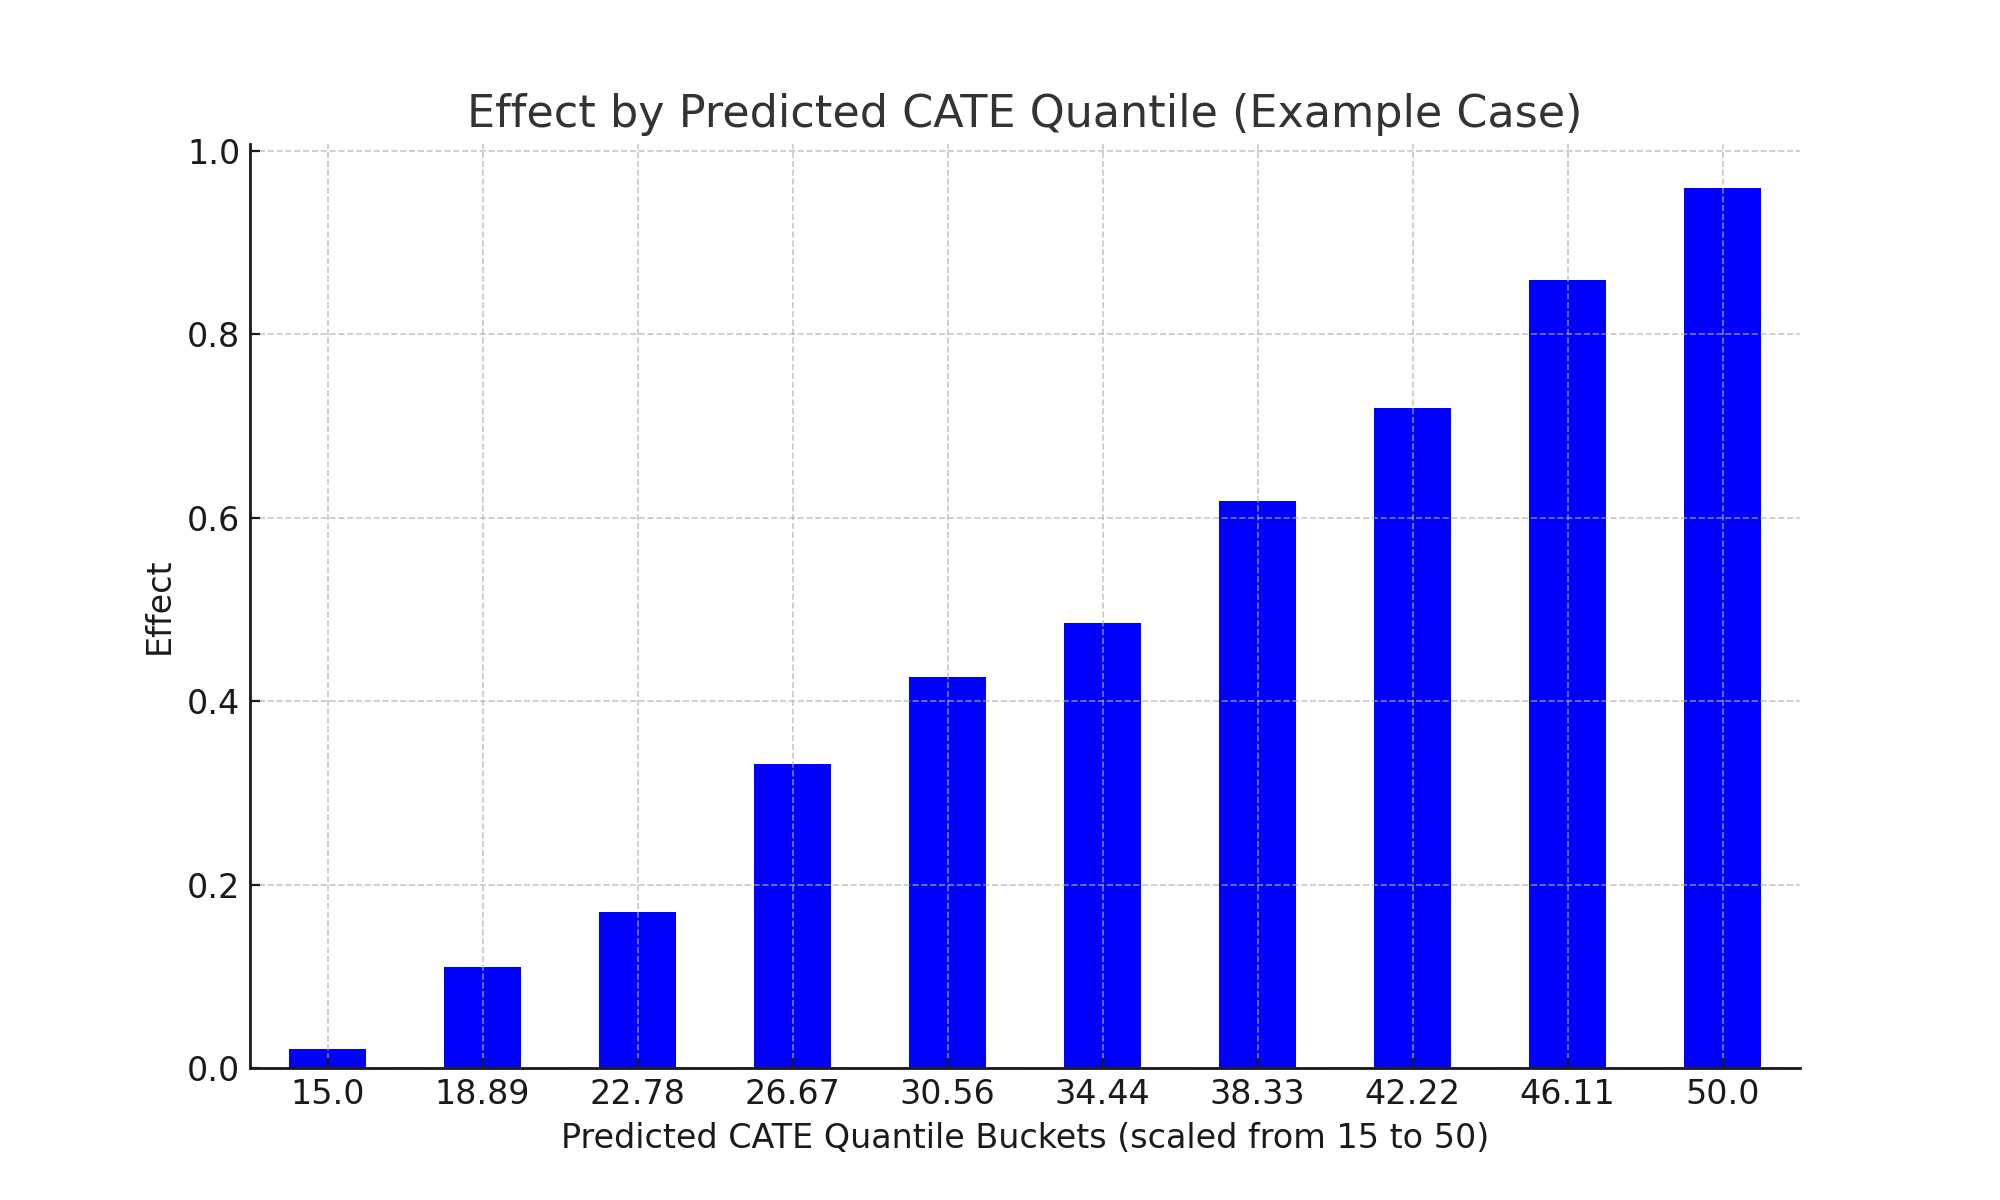
\includegraphics[height=2in]{effect_by_predicted_cate_quantile_example_case_rounded}
  \caption{Example of effect by CATE bucket}
  \label{fig:effect_by_quantile}
\end{figure}

A key challenge in this type of evaluation is the difficulty in comparing different models. Ideally, there would be a single metric that summarizes a model’s performance in correctly ranking the true heterogeneous effect (\gls{CATE}).
To address this, a first step is to calculate the cumulative effect across the buckets of predicted \gls{CATE}. This estimate would provide an idea of the concentration of the causal effect, allowing us to understand the accumulated causal 
effect in the top predicted CATE buckets.

In most cases, this cumulative causal effect tends to be concentrated in buckets with few individuals, which increases the uncertainty of the causal effect estimate in these buckets due to the small sample size. An alternative is to weight 
the estimates of the buckets by the number of individuals in each bucket, the resulting curve is known as the Cumulative Gain Curve. To make it more interpretable, it is common to divide it by the average predicted causal effect, thus being 
called the Relative Cumulative Gain Curve.

With the cumulative gain curve constructed, it is possible to estimate the area under this curve, thus, this metric represents how well the causal model ranks individuals according to their predicted \gls{CATE}. It is important to note that 
the area under the cumulative gain curve does not indicate how accurate or calibrated the predicted \gls{CATE} estimates are; rather, it reflects the model’s ability to rank them correctly.

This metric provides an overall view of the model’s performance but does not offer insight into individual performance. Some metrics in the literature attempt to address this point, such as the DR-Score and others discussed in \textcite{mahajan_empirical_2023}.
In the context of this study, developing a model capable of correctly ranking the \gls{CATE} meets the business needs and problem-solving requirements. However, having calibrated \gls{CATE} estimates would also contribute to the development of optimized policies and should
be considered as a future step within the scope of this thesis.

\subsection{Applications on marketing industry}
\label{sub:applications_marketing}

Uplift modeling has been increasingly applied in marketing to drive revenue growth through targeted advertising campaigns. Below are notable examples of how uplift modeling has been used to enhance marketing strategies.

\textcite{hansotia_incremental_2002} applied the UpliftVMA algorithm to examine consumer responses to promotional offers. In their study, a major U.S. retailer’s customers were randomly assigned to receive promotional mail. The effectiveness of the uplift approach was compared to
logistic regression models. The results demonstrated that the uplift model outperformed the top decile model and other traditional methods by more accurately predicting which customers would respond positively to the promotion.

\textcite{Radcliffe2007UsingCG} focused on customer retention by evaluating a company’s efforts to reduce churn through targeted incentives. By using uplift modeling, the company could identify customers who were likely to respond to retention efforts, resulting in significant improvements
in customer retention rates. This approach enabled the company to allocate resources more efficiently by focusing on customers most likely to be influenced by the retention efforts.

\textcite{blog_post} involved a direct marketing campaign where customers were divided into three groups: one receiving a men’s clothing promotion, another receiving a women’s clothing promotion, and a control group receiving no promotion. Uplift modeling was used to analyze the campaign’s 
impact on purchasing behavior. The study found that the uplift model could identify segments of customers who showed increased purchasing activity due to the targeted email advertisements, thus validating the model’s effectiveness in optimizing marketing strategies.

\textcite{van_der_aalst_random_2012} conducted a study on a Canadian insurance company to understand how uplift modeling could enhance cross-sell strategies. The company aimed to sell new insurance products to existing customers by targeting those likely to purchase additional coverage. 
By implementing uplift modeling, the company achieved a more significant increase in cross-sell success rates compared to traditional targeting methods. This demonstrated the model’s capability to improve marketing outcomes by identifying customers most likely to respond favorably to cross-selling efforts.

These examples illustrate the practical applications and benefits of uplift modeling in marketing. By focusing on individuals who are more likely to respond to specific marketing actions, companies can optimize their advertising efforts, increase customer engagement, and drive higher revenue growth. 
The success of these models in various marketing scenarios underscores their value in creating more effective and efficient marketing strategies.




